\documentclass[review]{elsarticle}

\makeatletter
\def\ps@pprintTitle{%
 \let\@oddhead\@empty
 \let\@evenhead\@empty
 \def\@oddfoot{\centerline{\thepage}}%
 \let\@evenfoot\@oddfoot}
\makeatother

\usepackage{lineno}
\usepackage[hyperfootnotes=false]{hyperref}
\usepackage{array, pbox}
\usepackage{mathtools}
\usepackage{caption}
\usepackage{graphicx}
\usepackage{subcaption}
\usepackage{CJKutf8}
\usepackage[page, titletoc, title]{appendix}
% \usepackage{tablefootnote}
\usepackage{threeparttable}
\usepackage{etoolbox}
\appto\TPTnoteSettings{\footnotesize}
\usepackage[bottom]{footmisc}
\usepackage{titling}


%to have numbered 4th level sections 1.1.1.1
\setcounter{tocdepth}{4}
\setcounter{secnumdepth}{4}

% to remove period in 4th level sections 1.1.1.1
\makeatletter
\def\els@aparagraph[#1]#2{\elsparagraph[#1]{#2}}
\def\els@bparagraph#1{\elsparagraph*{#1}}
\makeatother
% to enter a newline after 4th level sections
\newcommand{\myparagraph}[1]{\paragraph{#1}\mbox{}\smallskip}


\modulolinenumbers[5]

\journal{Nagaoka University of Technology}

%%%%%%%%%%%%%%%%%%%%%%%
%% Elsevier bibliography styles
%%%%%%%%%%%%%%%%%%%%%%%
%% To change the style, put a % in front of the second line of the current style and
%% remove the % from the second line of the style you would like to use.
%%%%%%%%%%%%%%%%%%%%%%%

%% Numbered
%\bibliographystyle{model1-num-names}

%% Numbered without titles
%\bibliographystyle{model1a-num-names}

%% Harvard
%\bibliographystyle{model2-names.bst}\biboptions{authoryear}

%% Vancouver numbered
%\usepackage{numcompress}\bibliographystyle{model3-num-names}

%% Vancouver name/year
%\usepackage{numcompress}\bibliographystyle{model4-names}\biboptions{authoryear}

%% APA style
%\bibliographystyle{model5-names}\biboptions{authoryear}

%% AMA style
%\usepackage{numcompress}\bibliographystyle{model6-num-names}

%% `Elsevier LaTeX' style
\bibliographystyle{elsarticle-num}
%%%%%%%%%%%%%%%%%%%%%%%

\begin{document}


%%%%%%%%%% cover page %%%%%%%%%%%

\begin{titlingpage}

\begin{centering}

\Large{
Nagaoka University of Technology
}

\bigskip

\large{
Graduate School of Engineering
}

\bigskip

\large{
Department of Information and Management Systems Engineering
}

\bigskip
\bigskip
\bigskip
\bigskip
\bigskip
\bigskip
\bigskip

\title{Analysis of Emotional Judgement factors based on online reviews from tourists visiting Japan}
\textbf{
\Large{
Analysis of Emotional Judgement factors based on online reviews from tourists visiting Japan
}}
\bigskip
\bigskip


\begin{CJK}{UTF8}{min}
(訪日観光客のオンラインレビューに基づく感情決定要因分析)
\end{CJK}

% \bigskip
% \bigskip

\bigskip
\bigskip
\bigskip
\bigskip
\bigskip
\bigskip
\bigskip

\normalsize{
A thesis submitted in partial fulfilment of the requirement for the degree of Master of Engineering, January 2019.
}
\bigskip

Submitted by

\textbf{
\large{
Alemán Carreón Elisa Claire
}}

\bigskip

\textbf{
Student No. 15340089
}
\bigskip
\bigskip

Supervised by
\medskip

\textbf{
\large{
Professor Hirofumi Nonaka
}}

\end{centering}

\end{titlingpage}

\clearpage
\thispagestyle{empty}
\tableofcontents{}
\clearpage

\setcounter{page}{1}

\linenumbers

\section*{Abstract}
In recent years there has been a boom in international tourism in Japan, where recently there has been particularly an increasing number of Chinese tourists, among other international tourists. In response to this boom and its effect on the Japanese economy, there is a need for the development of market research tools that are cost and time effective and rely on the advantages of online reviews, which increasingly affect sales and the influx of potential customers alike. In contrast with previous research, there is a need to use these online reviews to determine emotional judgement factors, words that most closely reflect the demands of these customer bases and the emotional judgement attached to them. Using an entropy-based mathematical model and a machine learning algorithm, I determined a set of keywords representing these emotional judgement factors. With this method, I extracted the most influential keywords in emotional judgement from Chinese and English online reviews of Japanese hotels in the portal sites \textit{Ctrip} and \textit{TripAdvisor}. I identified that Chinese customers react positively to included breakfasts and big rooms, and that unsatisfied Chinese customers focus on the pricing of the hotel. Additionally, I found that cheaper hotels have a focus on transportation, compared to luxury hotels. I also found English speaking customers dislike pricey hotels and have a high dislike for dirty rooms and stains, and that they mainly focus positively on staff, cleanliness, and transportation availability. Because the process is based on probabilistic distributions and automatic algorithms, it has potential future applications in cross-language businesses, especially the hospitality industry where language barriers are a constant problem.

\section{Introduction}\label{intro}

The population of Chinese tourists has recently increased significantly worldwide over the years. This increase has led to a significant impact on several industries over the world, most directly the hotel industry, as their customer bases changed. In addition to this impact on business, there is a current increase in academic research across the world about Chinese tourist populations \cite{sun2017}. Particularly in Japan, however, international tourism has been increasingly exerting a stronger influence in the economy \cite{Jones2009}. There were notable increases in the Chinese tourist population in Japan of 107.3\% from 2014 to 2015, and a total number of tourists of 6,372,948 in 2016 \cite{jnto2017}. This increase in international tourism creates a need for cross-language, cost and time effective market research tools. In the hospitality industry, where language barriers are a constant problem, there are difficulties and costs when attempting to understand the needs of their customer base. 

Until recent years, most of these market studies are performed based on the results of surveys or interviews. Currently, however, there are data mining and text mining techniques which potentially have the advantage over surveys and interviews. During recent years, several studies have successfully proved the validity and potential of using text and data mining analysis in the business management field. A study classified different kinds of Social Media posts and the customer response from several U.S. pizza selling companies \cite{he2013}. Another study ranked products by using online reviews and sentiment analysis \cite{liu2017149}, while another used them to predict product sales \cite{fan201790}. Other uses for text mining techniques include patent document analysis, as was done in a study on patent scoring \cite{nonaka2014}, and another on the extraction of technological terminology in patents \cite{nonaka2012}. It has also been used in the tourism and hospitality field to predict hotel demand by using web traffic data \cite{yang2014} or to make recommender systems \cite{loh2003}. Data mining and text mining techniques can not only cheaply and quickly gather tens of thousands if not more samples, but the source of this extensive amount of information also can be thought to be unaltered by any part of the data extraction process. 

An important benefit of using data and text mining in the hospitality field is that because of the current behavior of the customers in the information age, where the searching, choosing and booking process involves reading online reviews, and where customers write online reviews depending on their satisfaction or dissatisfaction. Previous studies have found that there is a correlation between prominent reviews and sales figures \cite{basuroy2003, ye2009}. There are also studies showing the direct impact of online hotel reviews on consumer consideration, that is, the decision process of many customers is affected either positively or negatively because of the reviews, with a stronger impact for lesser known hotels \cite{vermeulen2009}. Online reviews give researchers access to large databases of unfiltered customers opinions without the need to ask directly via surveys or interviews, and they also provide an availability of data from tourists writing in many languages. It is because of this important impact the hotel reviews have to consumers, and the highly polarized emotional content these reviews hold that I have decided to use this data for analysis.

Many researchers have focused on studying the level of satisfaction of customers for predefined factors \cite[e.g.][]{balbi2018, kim2017362, truong2009, wu2009, shanka2004, kozak2002}, while others focus on motivation, choice or behavior \cite[e.g.][]{chang2008, romao2014, dongyang2015}. However, most of the studies rely on making inferences about the larger population based on predefined factors, instead of extracting the factors directly from the data without human intervention. Not only that but when examining international tourism, they are limited by language barriers. In my study, I aim to use the benefits of online reviews to mathematically extract the answer to these questions in a manner that doesn't rely on understanding the language to expand it further to a larger corpus. In addition, while most studies with text mining techniques and sentiment analysis techniques focus on either relevant topics or the sentiment value of reviews, this study merges both techniques to find the relevant topics tied to each emotional response.

In my study, I developed a text mining method to extract emotional judegment keywords and analyze the needs of Chinese customers of Japanese Hotels. I chose this combination of population and destination because I aim to develop a methodology that can be applied in any language and regardless of language barriers on a large scale. For comparison I chose to also study the reviews from English speaking people staying in Japan. The extracted emotional judegment keywords became the key to researching which topics and in what order of priority the general Chinese tourist population consider when they write their reviews. This is, of course, valuable information for making business management decisions from the point of view of the hotel industry companies. Knowing which topics are not only largely discussed, but those that are most related to customer satisfaction, a company can improve customer service or facilities to increase profit. Using the methodology detailed in this study, such knowledge can become available to other researchers and companies by applying it in different environments.

\section{Research Objective}\label{research_objective}

The objective of this study is to determine the factors influencing emotional judegment in the satisfaction or dissatisfaction of Chinese customers of Japanese Hotels because of the language barrier that can be studied and the economic weight that these customers represent, as well as studying English speaking tourist populations for comparison. These emotional judegment factors can become the focal point for making improvements in tourism and service industries, increase the satisfaction of customers, and influence newer customers to write more satisfied online reviews that will in turn increase sales and attract new customers. 

I aim to create a process that is based on probability distributions and automatic algorithms, and that is not dependent on language-specific methodologies that limit its application in other environments. To do this, I propose to use supervised machine learning to be trained on emotional judegment classification of online review texts and use it not only to classify other texts further but to analyze the weight towards classification that certain keywords hold in that trained machine. Furthermore, I also analyze the relevance of these keywords in different hotel price brackets to observe potential differences. 

\section{Related Work}\label{relatedwork}

In the hospitality field, satisfaction, motivation, and behavior have been studied for a long time using surveys \cite[e.g.][]{truong2009, wu2009, shanka2004, kozak2002, chang2008, romao2014, dongyang2015, chan201518}. More recently, studies have used big data in the hospitality industry \cite[e.g.][]{yang2014, loh2003}, as well as data mining tools to analyze hotel reviews \cite[e.g.][]{alsmadi2018, browning2013, xiang2010}. However, most focus on either the sentiment classification without analyzing the words influencing that emotion, or they study the words without taking the emotions into account. Other studies focus on review helpfulness \cite{ren2018}; while others focus on summarization of reviews into smaller text \cite[e.g.][]{hu2017436, amplayo201754}. There has not been yet a study that focuses on the conceptual words that lead directly to an emotional decision from the user. For example, one study used a tool called “Word Cloud” to extract frequently used words inside the reviews which were considered important topics of concern to consumers \cite{hargreaves2015}. However, the sentiment analysis is done at a hotel level, instead of a word level, so it is difficult to determine which topics are perceived positively or negatively. Another study used a heuristic frequency analysis to determine guest experience topics \cite{xiang2015}. However, this study doesn't deterministically show which topics directly influence satisfaction and dissatisfaction or the order in which they do.

On the other hand, Zhang et al. performed a market analysis based on the sentiment analysis of product reviews using a Chinese sentiment dictionary called HowNet \cite{zhang2011}. The problem with using HowNet as a sentiment dictionary is that the words are classified based on ontology \cite{huang2008}, where emotional words are usually those that describe emotions, such as “angry”, “anger”, “happiness”, “content”. While these words represent the emotions themselves, in an online review, it is unlikely that the general population writes their emotions explicitly; instead, it is more likely that words that do not describe the emotion but are intrinsically emotionally fueled are used. For example, one would not write “I am happy with the size of the room and the service”; instead what would be natural is “The room had lots of space for our luggage and the staff was friendly”. HowNet is not able to determine that “space” is positive and that “staff” is being praised by the use of “friendly” in the sentence. These non-emotional words are directly influencing the emotional judegment in the online review. Now, in turn, this study methodology focuses on the influence of each word and their rank of importance in relation to the emotional judegment taken by the user, clearly defining not only the emotions but also the specific needs of Chinese customers in a concrete way.

There have been previous attempts at understanding the factors leading to satisfaction and dissatisfaction with text and data mining techniques as well. One study used a text-link analysis to understand which pairs of words were used more in positive or negative reviews \cite{berezina2016}. However, the conclusions of this study are limited to their sample of manually classified 20 reviews, so it is difficult to extrapolate it to a larger population of reviews. Another study manually extracted factors that could lead to satisfaction or dissatisfaction from a sample and then continued to study the statistical differences between them in that sample \cite{zhou2014}. However, this is limited to their manually defined factors and that there are no further analyses to a larger number of online reviews because of language barriers. Another study used heuristic language-specific parsing algorithms to determine the frequency of words in a previously classified corpus \cite{xu2016}. The problem with this last method is that it is depending on the specific corpus of reviews classified as negative or positive from the moment they're input into the site into different input forms from \textit{Booking.com} and that it is strictly only applicable to English texts. My methodology not only applies the findings of the sampling to the full corpus, but it does in a way that overcomes the difficulties of language barriers and sentiment classification.

Previous research in the field of linguistics and psychology has been made in an effort to detect and classify emotion in Chinese texts, using emotional verbs and other linguistic features in texts \cite[e.g.][]{lee2010-b, chen2010emotion}. Many studies are mainly based on the Sinica Treebank \cite{chen1999}, Sinica Corpus \cite{huang1992}, Penn Chinese Treebank \cite{xue2005}, and Chinese Gigaword Corpus \cite{huang2005}, which contain texts on subjects like science, philosophy, literature, art, financial newsletters, articles, among other formal texts. While using these can be effective in classifying emotional states in similarly formal or literary texts, there are no appropriate training corpora for this current endeavor, which includes informal internet slang and a focus on service or product satisfaction. This is why I have decided to train my model using only the collected data. That is to say, the segmentation of Chinese words using these corpora has been done successfully in other hotel review studies \cite[e.g.][]{chen20181325}, and so I have decided to employ them as well.

\section{Methodology}\label{method}

I have extracted a large number of text reviews from a Chinese portal site \textit{Ctrip}\footnote{\label{ctrip}Ctrip: \href {www.ctrip.com/}{\path{www.ctrip.com/}}}, as well as the travel site \textit{TripAdvisor}\footnote{\label{tripadvisor}TripAdvisor: \href {www.tripadvisor.com/}{\path{www.tripadvisor.com/}}} and determined the most commonly used words that would contribute the most to emotional judegment behind positive and negative opinions in a review using an entropy-based mathematical extraction method. These keywords extracted using entropy related to emotional judegment not only allow us to perform a Support Vector Machine based emotional classification of the reviews but conceptual words in these lists bring insight into which concrete topics are the Chinese tourists concerned with. After classifying the sentences in the extracted reviews as positive and negative with an optimized SVM, I have analyzed the weight value assigned to them by the SVM. For words that are not part of the support vector this is equal to 0; however, the support vector lets us observe the words that, while potentially close to the border between positive and negative sentiments, provide a strong and clear distinction in the emotional classification. This will be explained further in section \ref{svmweightsanalysis}. These words, especially those signifying a subject or topic, allow us to analyze the writing tendencies of Chinese customers in either positive or negative reviews. I also observed the frequency of the terms in all of the reviews to extract the most utilized words in either kind of reviews. I show an overview of this methodology in Figure \ref{fig:method-overview}. I repeated this experiment in a corpus of reviws of Japanese hotels written in English for comparison. Furthermore, I have also performed analyses for different price brackets to observe the change in demand for different kinds of hotels varying in luxury in the Chinese reviews.

\begin{figure}[bp]
\centering
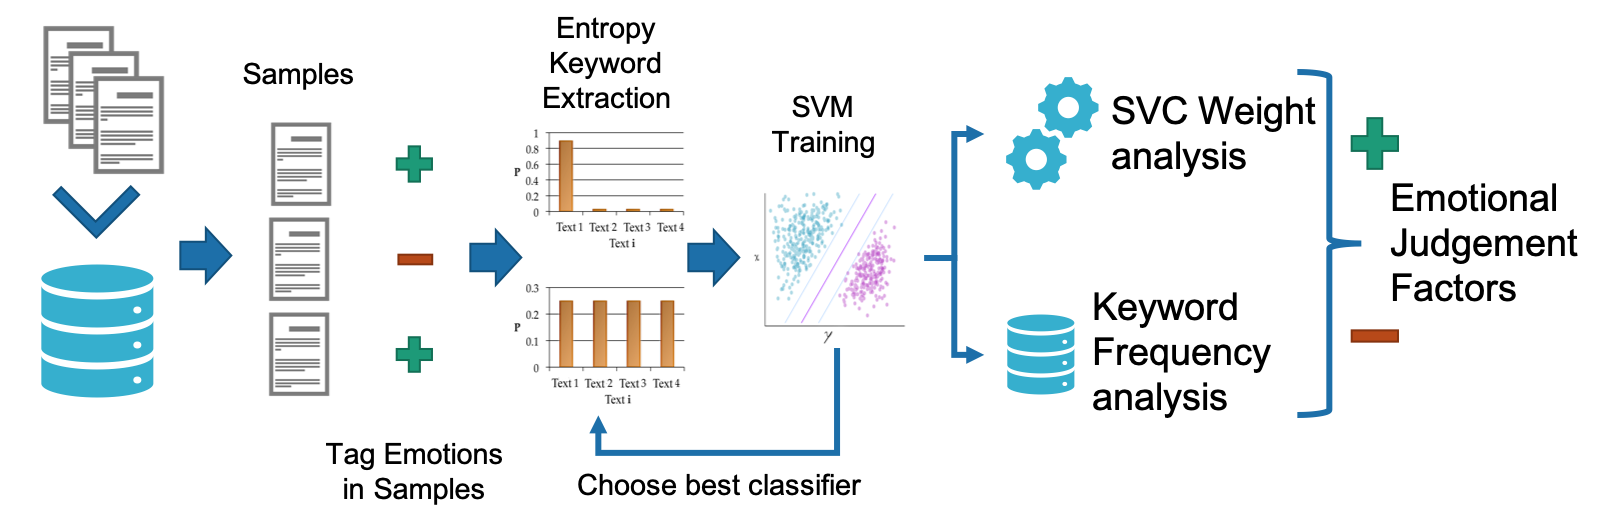
\includegraphics[width=\textwidth]{figures/method-overview.png}
\caption{Overview of the Methodology}
\label{fig:method-overview}
\end{figure}

\subsection{Data Collection}\label{datacollection}

In this study I used the HTML parsing python library \textit{BeautifulSoup}\footnote{\label{bs4}Beautiful Soup: \href {https://www.crummy.com/software/BeautifulSoup/}{\path{https://www.crummy.com/software/BeautifulSoup/}}}, and the local database management tool \textit{SQLite}\footnote{\label{sqlite}SQLite: A local database management system with an SQL structure: \href {https://www.sqlite.org/}{\path{https://www.sqlite.org/}}} using the python library \textit{sqlite3} to automatize data managing processes.

\subsection{Data Processing}\label{dataprocessing}

\subsubsection{Text Processing}\label{textprocessing}

Different from the English language, Chinese texts lack a separation between different words, and as such, when collecting these texts, they are all a single string of characters. To be able to perform a statistical analysis of each word, the Stanford Word Segmenter \cite{chang2008} program developed by the Stanford NLP Group\footnote{\label{stanfordnlp}The Natural Language Processing Group at Stanford University} was implemented for this task using the python \textit{nltk} library. During the segmentation of all the words in my corpus, irregularities occurred where the reviews were written in other languages or where unusual punctuation marks were used. I designated a list of characters that could be recognized as noise, such as punctuation marks, then cleared all the text in the corpus of these characters. 

In the case of English text, however, only using spaces is not enough to correctly collect concepts. Because of variations and conjugations of words depending on the context and tense, a better segmentation is achieved by using lemmatization, which returns the dictionary form of each word. For this purpose I used the \textit{gensim} library with the English texts.

\subsubsection{Sentiment Analysis}\label{sentimentanalysis}

\myparagraph{Entropy Based Keyword Extraction}\label{entropy}

In order to determine the words that clearly impact the user’s emotional judegment, I calculated the entropy value of each word in relation to each class. Shannon’s Entropy, in the field of Information Theory, is defined to be the expected value of the information content in a signal \cite{shannon1948} or it can be thought of as the grade of impossibility of predicting an outcome. Using this value I can observe the probability distribution of each word inside the corpus. A word that is included in many documents, it will have a high entropy value for that set of documents, since it becomes uncertain to predict in which document it will appear. Opposite to this, a word appearing in only one document will have an entropy value of zero, since it is completely predictable. I show this concept in Figure \ref{fig:entropygraphs}.

\begin{figure}[bp]
	\centering
	\begin{subfigure}[b]{0.4\linewidth}
		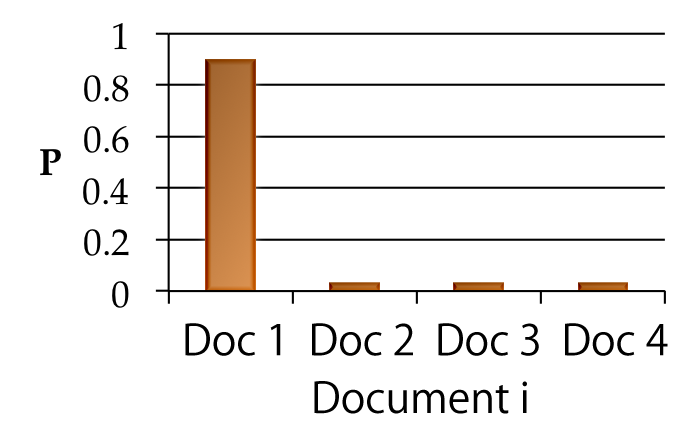
\includegraphics[width=\linewidth]{figures/entropyzero.png}
		\caption{Entropy close to zero}
	\end{subfigure}
	\begin{subfigure}[b]{0.4\linewidth}
		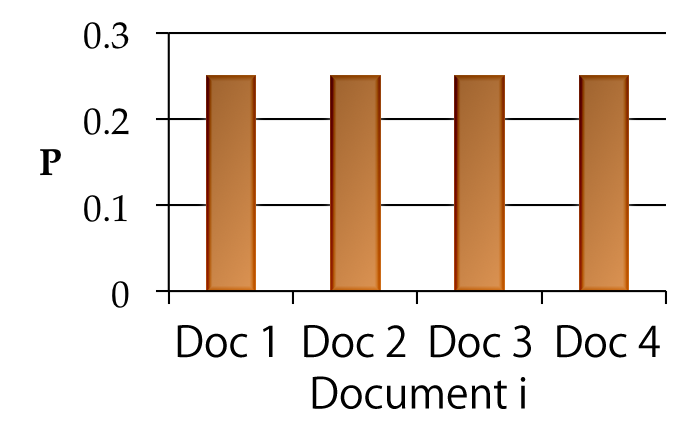
\includegraphics[width=\linewidth]{figures/entropyhigh.png}
		\caption{High entropy}
	\end{subfigure}
\caption{Probabilities of a word j being contained in a document i}
\label{fig:entropygraphs}
\end{figure}

To apply this logic, I retrieved 50 reviews as a sample of my corpus and with the collaboration of a group of 5 Chinese students, tagged each sentence of a total of 159 as the classes positive or negative depending on the emotion that the text conveyed, then calculated the entropy values for each word in relation to the set of sentences from each class. In the case of English reviews, I sampled 665 reviews and with the collaboration of English speaking students manually tagged them by sentence, resulting in 2357 tagged sentences. Words with higher entropy relating to the positive set than to the negative set by a factor of \(\alpha\) were determined to be keywords influencing positive emotional judegment in Chinese reviews of hotels. Likewise, words with higher entropy for the negative set than the positive set by a factor of \(\alpha'\) were determined to be keywords related to the negative emotional judegment in my texts. 

In the formulas below I show my process for the calculation the the entropy of each word \(i\) in each document \(j\) in the positive set of documents \(H_{Pj}\) (\ref{eq:Hpj}) and the entropy for the negative set \(H_{Nj}\) (\ref{eq:Hnj}) below, using the probabilities of a word being in a positive document \(P_{ijP}\) (\ref{eq:PijP}) and likewise for negative documents \(P_{ijN}\) (\ref{eq:PijN}). \(N_{ijP}\) is the number of times a word \(i\) is included in a document \(j\) from the positive set and likewise for \(N_{ijN}\) with regard to the negative set. Lastly I show the keyword determining comparison formula using the mutually independent coefficients \(\alpha\) and \(\alpha'\) in the formulas (\ref{eq:entropy_pos}) and (\ref{eq:entropy_neg}) respectively.

\begin{equation}\label{eq:Hpj}
H_{Pj} = - \sum_{i=1}^M [P_{ijP}\log_2 P_{ijP}]
\end{equation}

\begin{equation}\label{eq:lim_Hpj}
\lim_{P_{ijP}\to0+} P_{ijP}\log_2 P_{ijP} = 0
\end{equation}

\begin{equation}\label{eq:Hnj}
H_{Nj} = - \sum_{i=1}^M [P_{ijN}\log_2 P_{ijN}]
\end{equation}

\begin{equation}\label{eq:lim_Hnj}
\lim_{P_{ijN}\to0+} P_{ijN}\log_2 P_{ijN} = 0
\end{equation}

\begin{equation}\label{eq:PijP}
P_{ijP} = \frac{N_{ijP}}{\sum_{i=1}^M N_{ijP}}
\end{equation}

\begin{equation}\label{eq:PijN}
P_{ijN} = \frac{N_{ijN}}{\sum_{i=1}^M N_{ijN}}
\end{equation}

\begin{equation}\label{eq:entropy_pos}
H_{Pj} > \alpha H_{Nj}
\end{equation}

\begin{equation}\label{eq:entropy_neg}
H_{Nj} > \alpha' H_{Pj}
\end{equation}

\myparagraph{Support Vector Machine Classification}\label{svm}

Support Vector Machines are supervised machine learning models usually applied to classification or regression problems \cite{cortes1995}. I use it to classify the rest of my corpus into emotional classes in my study. An SVM is trained to classify data based on previously labeled data, generalizing features of the data by defining a separating (p-1)-dimensional hyperplane in a p-dimensional space in which each dimension is a feature of the data. The separating hyperplane, along with the support vectors, divides the multi-dimensional space and minimize the error of classification. I show a two dimensional example in Figure \ref{fig:svm2d}.

\begin{figure}[bp]
\centering
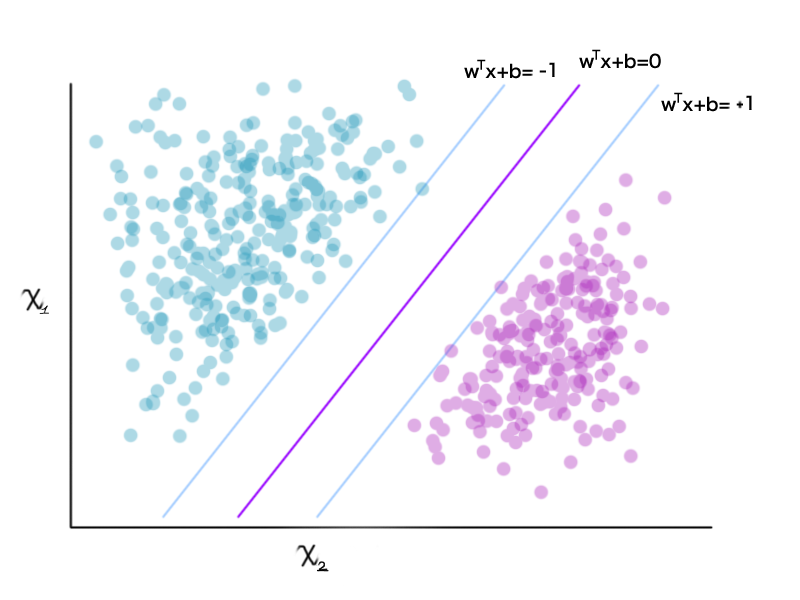
\includegraphics[width=20em]{figures/SVM_2d_example.png}
\caption{Two dimensional example of an SVM classification problem}
\label{fig:svm2d}
\end{figure}

In my study, I used the linear kernel of the SVM classification process, defined by the formula (\ref{eq:svm1}) below. Each training sentence is a point of data, a row in the vector \(x\), where each column represents a feature, in my case the quantities of each of the keywords in that particular sentence. The labels of previously known classifications (1 for positive, 0 for negative) for each sentence comprise the \(f(x)\) vector. The Weight Vector \(w\) is comprised of the influences each point has had in the training process to define the angle of the hyperplane and the bias coefficient \(b\) determines its position, as explained in section \ref{svmweightsanalysis}. After the hyperplane is drawn, the classification of the new data is done as follows in formula (\ref{eq:svm2}) and (\ref{eq:svm3}).

\begin{equation}\label{eq:svm1}
f(x) = w^\top x + b
\end{equation}

\begin{equation}\label{eq:svm2}
f(x_{new})\geq 0 \rightarrow y_{new} = +1 
\end{equation}

\begin{equation}\label{eq:svm3}
f(x_{new})\leq 0 \rightarrow y_{new} = -1 
\end{equation}

At the beginning of the process, the initial weights for each word are set to zero. Then, as a random separating vector is drawn, each data point \(x_i\) is tested and if the classification for it fails, the value for \(w\) is changed by a value of \(\alpha\) as follows (\ref{eq:svm4}). This \(\alpha\) is not to be confused with the entropy comparison \(\alpha\) and \(\alpha'\) in section \ref{entropy}.

\begin{equation}\label{eq:svm4}
w \leftarrow w + \alpha sign(f(x_i))x_i
\end{equation}

The process is then repeated until the classification error is minimized as much as possible. The resulting function for classification can be expressed as follows (\ref{eq:svm5}). In the end, although the weight vector is the same size as the number of feature words, weight is only assigned to words that are explicitly inside the support vectors that are close to and guide the separating hyperplane.

\begin{equation}\label{eq:svm5}
f(x) = \sum_{i=1}^N \alpha_i y_i (x_i^\top \cdot x) + b
\end{equation}

In the field of corpus study and Natural Language Processing, each of the features of a data point is the number of times that a word is included in a document. In my study I used a number of keyword lists, defined by my entropy calculations with different comparison coefficients, as the possible features; trained the SVMs implementing the Support Vector Classifier included in the python library \textit{scikit-learn}\footnote{\label{scikitlearn}Scikit-Learn \href {http://scikit-learn.org/}{\path{http://scikit-learn.org/}}}; managed the vector mathematics with the mathematical python library \textit{numpy}\footnote{\label{numpy}Numpy. \href {http://numpy.org/}{\path{http://numpy.org/}}}; and tested for each one using the K-fold Cross-Validation method, which has been proven to provide good results in small samples \cite{kohavi1995}. In each test I calculated the Precision, Recall and \(F_1\)-measure \cite{powers2011} for my predictions.

\myparagraph{Model Evaluation Metrics}
\label{model_evaluation}

In order to measure the effectiveness of the training process and data, I performed what is called a K-fold cross-validation. This means that after randomly shuffling and splitting my training data into k equal parts, k-1 of those parts are used for training, while the remaining one part is used in validation. Using the trained models, a prediction is made, and it is decided if such a prediction is correct or not, and counted and grouped as a True Positive, True Negative, False Positive or False Negative prediction. This is explained in Table \ref{tab:preds}.

\begin{table}[bp] \centering
\caption{Prediction outcomes}\label{tab:preds}
\begin{tabular}{c|c|c|}
\cline{2-3}
\textbf{} & \textbf{Prediction is Correct} & \textbf{Prediction is Incorrect} \\ \hline
\multicolumn{1}{|c|}{\textbf{\begin{tabular}[c]{@{}c@{}}Prediction\\  is Positive\end{tabular}}} & True Positive & False Positive \\ \hline
\multicolumn{1}{|c|}{\textbf{\begin{tabular}[c]{@{}c@{}}Prediction \\ is Negative\end{tabular}}} & True Negative & False Negative \\ \hline
\end{tabular}
\end{table}

Measures of accuracy are determined from these prediction outcomes. This process is then repeated \(k\) times and the measures taken are averaged. In this study, I used the \(F_{1}\) score, which measure is a harmonic mean between precision and recall. Precision, described in formula (\ref{eq:precision}), lets us observe the rate of correct positive predictions from all the positive predictions, while Recall, detailed in formula (\ref{eq:recall}), observes the rate of correct positive predictions from the total of actual positive data. The \(F_{1}\) score in formula (\ref{eq:f1}) then can only be high when both of these measures are high simultaneously and will lower substantially if they are not consistent. I use this score as it allows us to avoid overlooking data while maintaining accurate predictions. The overall accuracy (\ref{eq:accuracy}), which doesn't account for overlooking of data, is also observed for reference but isn't used as the main evaluation of the model.

\begin{equation}\label{eq:precision}
Precision = \frac{True Positives}{True Positives + False Positives}
\end{equation}

\begin{equation}\label{eq:recall}
Recall = \frac{True Positives}{True Positives + False Negatives}
\end{equation}

\begin{equation}\label{eq:f1}
F_{1} = 2  \frac{Precision * Recall}{Precision + Recall}
\end{equation}

\begin{equation}\label{eq:accuracy}
Accuracy = \frac{True Positives + True Negatives}{Number Of Predictions}
\end{equation}

\subsubsection{Data Analysis}\label{dataanalysis}

\myparagraph{SVM Weight Analysis}\label{svmweightsanalysis} 

As stated earlier in section \ref{svm}, each point of data that is classified incorrectly causes a change in the weight vector to better locate the separating hyperplane and classify new data correctly. These changes to the weight vector are strong for features that needed to be taken account of to classify with a minimal error, those contained in the support vectors, close to the separating hyperplane. Sequentially, the weight vector can be interpreted as a numerical representation of the effect each feature, or in my case, each of these normally ambiguous words, had for the classification process and the class it has a decisive influence in. Because the weight vector gives value to the words that comprise the support vectors, the words with higher weights are thought to be closer to the dividing hyperplane, while still clearly and decisively belonging to one of the categories the hyperplane divides the high-dimensional space in. While other less ambiguously used words could be excluded from this weight assigning process, the words that are assigned weight values are thought to be words that while discussed in both emotional states, they are more strongly discussed in one of these emotional states. If anything, these are highly volatile words relating to the experience of the customers in the hotel, which are important to consider as a hotel business to improve customer satisfaction. Below I show the formula for the weight vector (\ref{eq:svm_weight}).

\begin{equation}\label{eq:svm_weight}
w = \sum_{i=1}^N \alpha_i y_i x_i
\end{equation}

\myparagraph{Keyword Frequency Analysis}\label{keywordfrequencyanalysis}

Because the machine learning model used in my study is constructed from training data obtained by a relatively small sample of my data, after training the model and classifying the rest of my data, I studied the frequencies of each entropy based keyword in my complete data set. Words signifying a subject or topic that are relatively highly used will have more meaning when analyzing the emotional response of the user-base of Chinese tourists in Japan. Keywords with lower frequencies can be interpreted to be emotional keywords to a small sector of the user-base, but this information is important nevertheless from a mathematical and a marketing standpoint.

\section{Results}\label{results}

\subsection{Data set}\label{dataset}

In my data collection stage a total of 1,541,424 html files were crawled, from which 5,938 were unique review pages of hotels in Japan. From these pages, I extracted a total of 44,912 reviews, which were comprised of 286,109 separate sentences. In my corpus, there were 23,443 different words used, from which 2,802 were noise characters.

\subsection{Sentiment Analysis Results}\label{sentimentresults}

After having my training data tagged by a group of 5 Chinese student collaborators, I experimented with different comparison coefficients for the entropy values calculated from the ‘positive’ and ‘negative’ emotional classes. The mutually independent coefficients \(\alpha\) and \(\alpha'\) were tested from 1.25 to 6 in intervals of 0.25. The result was 40 lists, 20 for each emotional class. I repeated the process for the reviews in English that my colleagues tagged.

In the beginning, I experimented with different kernels for the SVM, as well as some Ensemble Learning methods, like the Boosting, Voting and Stacking. I ultimately decided to use the linear kernel for the benefits of the weight vector obtainability. I also experimented with different parameters for the SVC, finding that the best performing value for C, a constant that affects the optimization process when minimizing the error of the separating hyperplane. Low values of C give some freedom of error, which minimizes false positives, but depending on the data it can increase false negatives. Inversely, high values of C will likely result in minimal false negatives, but a possibility of false positives. I found the ideal value for this parameter was C=0.5 in my final classifier for Chinese text, and 2 in the English text one.

I trained a different Support Vector Classifier with each of the lists, and I chose the best performing lists for each emotional class, resulting in a positive emotion classifier (positive or not positive) and a negative emotion classifier (negative or not negative), based on the results of a 5-fold cross-validation process in the Chinese reviews, and a 10-fold cross-validation process in the English reviews case, in which I calculated their accuracy and F-measure means and standard deviations. The number of \(k\)-folds was decided from the sample size. Since the sample for the Chinese texts was smaller, the number of validation data would be reduced if a higher value for \(k\) was used. After observing the misclassification behavior for the positive emotion classifier, which mostly misclassified sentences with negative words, I decided to combine both keyword lists into a single large list to train the positive emotion classifier. With this Combined list, the accuracy was of \(0.92 \pm 0.03\) and \(F_1 = 0.95 \pm 0.01\), both excellent results for classification. Table \ref{tab:svm_f1_zh} shows the lists that had the best performance results in the case of Chinese text and Table \ref{tab:svm_f1_en} shows the best performance results in English texts.

\begin{table}[bp] \centering
\caption{Results of the best 5-fold Cross-Validation Chinese text classification performance tests}\label{tab:svm_f1_zh}
\resizebox{\textwidth}{!}{%
\begin{tabular}{|l|l|l|l|l|l|l|}
\hline
Keyword List & \begin{tabular}[c]{@{}l@{}}Classifier \\ emotion\end{tabular} & C & \begin{tabular}[c]{@{}l@{}}Accuracy \\ \(\mu\)\end{tabular} & \begin{tabular}[c]{@{}l@{}}Accuracy\\  \(\sigma\)\end{tabular} & \begin{tabular}[c]{@{}l@{}}\(F_1\) \\ \(\mu\)\end{tabular} & \begin{tabular}[c]{@{}l@{}}\(F_1\) \\ \(\sigma\)\end{tabular} \\ \hline
\begin{tabular}[c]{@{}l@{}}Positive keywords \\ (\(\alpha=2.75\))\end{tabular} & \begin{tabular}[c]{@{}l@{}}Positive \\ emotion\end{tabular} & 2.5 & 0.87 & 0.02 & 0.91 & 0.01 \\ \hline
\begin{tabular}[c]{@{}l@{}}Negative keywords \\ (\(\alpha'=3.75\))\end{tabular} & \begin{tabular}[c]{@{}l@{}}Negative \\ emotion\end{tabular} & 0.5 & 0.85 & 0.05 & 0.67 & 0.11 \\ \hline
\begin{tabular}[c]{@{}l@{}}\textbf{Combined} \\ (\(\alpha\)=2.75, \(\alpha'\)=3.75)\end{tabular} & \textbf{\begin{tabular}[c]{@{}l@{}}Positive \\ emotion\end{tabular}} & \textbf{0.5} & \textbf{0.92} & \textbf{0.03} & \textbf{0.95} & \textbf{0.01} \\ \hline
\end{tabular}%
}
\end{table}

\begin{table}[bp] \centering
\caption{Results of the best 10-fold Cross-Validation English text classification performance tests}\label{tab:svm_f1_en}
\resizebox{\textwidth}{!}{%
\begin{tabular}{|l|l|l|l|l|l|l|}
\hline
Keyword List & \begin{tabular}[c]{@{}l@{}}Classifier \\ emotion\end{tabular} & C & \begin{tabular}[c]{@{}l@{}}Accuracy \\ \(\mu\)\end{tabular} & \begin{tabular}[c]{@{}l@{}}Accuracy\\  \(\sigma\)\end{tabular} & \begin{tabular}[c]{@{}l@{}}\(F_1\) \\ \(\mu\)\end{tabular} & \begin{tabular}[c]{@{}l@{}}\(F_1\) \\ \(\sigma\)\end{tabular} \\ \hline
\begin{tabular}[c]{@{}l@{}}Positive keywords \\ (\(\alpha=1.5\))\end{tabular} & \begin{tabular}[c]{@{}l@{}}Positive \\ emotion\end{tabular} & 1.75 & 0.79 & 0.02 & 0.82 & 0.02 \\ \hline
\begin{tabular}[c]{@{}l@{}}Negative keywords \\ (\(\alpha'=4.25\))\end{tabular} & \begin{tabular}[c]{@{}l@{}}Negative \\ emotion\end{tabular} & 3 & 0.70 & 0.04 & 0.80 & 0.03 \\ \hline
\begin{tabular}[c]{@{}l@{}}\textbf{Combined} \\ (\(\alpha\)=1.5, \(\alpha'\)=4.25)\end{tabular} & \textbf{\begin{tabular}[c]{@{}l@{}}Positive \\ emotion\end{tabular}} & \textbf{2} & \textbf{0.81} & \textbf{0.02} & \textbf{0.83} & \textbf{0.02} \\ \hline
\end{tabular}%
}
\end{table}

Using both sets of keywords in the same SVC (named ‘Combined’) to classify my testing data, I obtained higher performance results overall. I then used these classifiers in the rest of the respective data to label positive emotion sentences. The sentences not belonging to the positive emotion class were considered to belong in the negative emotion class since the classification of the emotion of each sentence was binary in my training samples original classification.

\subsection{Keywords and their SVM Weight Values}\label{svmresults}

In Table \ref{tab:key_weights_zh} I show some of my keywords that signify subjects or topics, and as such, help us understand the needs of the users. I show keywords that have a relatively high weight value for both positive and negative extremes, and their translations in the relevant context. In Table \ref{tab:key_weights_en} I show keywords for the English classifier with high weight values.

\begin{table}[bp] \centering
\caption{High weight values for Chinese keywords signifying subjects or topics}
\label{tab:key_weights_zh}
\begin{tabular}{|>{\centering\arraybackslash}m{3em}|m{10em}|>{\centering\arraybackslash}m{4em}|>{\centering\arraybackslash}m{5em}|} \hline
\textbf{Word} & \multicolumn{1}{c|}{\textbf{Translation}} & \textbf{Entropy List} & \textbf{SVC Weight} \\ \hline
\begin{CJK}{UTF8}{gbsn} 地方 \end{CJK} 
    & region, local 
        & positive 
        & 1.343 \\ \hline
\begin{CJK}{UTF8}{gbsn} 干净 \end{CJK} 
    & clean 
        & positive 
        & 0.638 \\ \hline
\begin{CJK}{UTF8}{gbsn} 大 \end{CJK} 
    & big, wide 
        & positive 
        & 0.624 \\ \hline
\begin{CJK}{UTF8}{gbsn} 交通 \end{CJK} 
    & traffic, transportation 
        & positive 
        & 0.586 \\ \hline
\begin{CJK}{UTF8}{gbsn} 热情 \end{CJK} 
    & cordial, kindness 
        & positive 
        & 0.495 \\ \hline
\begin{CJK}{UTF8}{gbsn} 周边 \end{CJK} 
    & periphery 
        & positive 
        & 0.495 \\ \hline
\begin{CJK}{UTF8}{gbsn} 景色 \end{CJK} 
    & scenery 
        & positive 
        & 0.495 \\ \hline
\begin{CJK}{UTF8}{gbsn} 推荐 \end{CJK} 
    & recommendation 
        & positive 
        & 0.495 \\ \hline
\begin{CJK}{UTF8}{gbsn} 日本 \end{CJK} 
    & Japan 
        & positive 
        & 0.495 \\ \hline
\begin{CJK}{UTF8}{gbsn} 早餐 \end{CJK} 
    & breakfast 
        & positive 
        & 0.495 \\ \hline
\begin{CJK}{UTF8}{gbsn} 附近 \end{CJK} 
    & nearby 
        & positive 
        & 0.495 \\ \hline
\begin{CJK}{UTF8}{gbsn} 中文 \end{CJK} 
    & Chinese text 
        & negative 
        & -0.714 \\ \hline
\begin{CJK}{UTF8}{gbsn} 地理 \end{CJK} 
    & geography 
        & negative 
        & -0.812 \\ \hline
\begin{CJK}{UTF8}{gbsn} 价格 \end{CJK} 
    & price 
        & negative 
        & -1.505 \\ \hline
\end{tabular}
\end{table}

\begin{table}[bp]
\centering
\caption{High weight values for English keywords signifying subjects or topics}
\label{tab:key_weights_en}
\begin{tabular}{|l|c|c|}
\hline
\multicolumn{1}{|c|}{\textbf{Word}} & \multicolumn{1}{c|}{\textbf{\begin{tabular}[c]{@{}c@{}}Entropy\\ List\end{tabular}}} & \multicolumn{1}{c|}{\textbf{SVC Weight}} \\ \hline
bathhouse & Positive & 2.000 \\ \hline
museum & Positive & 2.000 \\ \hline
meeting & Positive & 1.997 \\ \hline
subway & Positive & 1.951 \\ \hline
cozy & Positive & 2.000 \\ \hline
convenience & Positive & 1.888 \\ \hline
clean & Positive & 1.886 \\ \hline
comfortable & Positive & 1.724 \\ \hline
dirty & Negative & -1.275 \\ \hline
policy & Negative & -1.463 \\ \hline
prepay & Negative & -1.517 \\ \hline
pricey & Negative & -1.614 \\ \hline
sticky & Negative & -2.000 \\ \hline
\end{tabular}
\end{table}

\subsection{Keyword Frequencies}\label{freqresults}

I observed the words with the highest frequencies for keywords in positive and negative statements to study the needs of Chinese customers, as shown in the Tables \ref{tab:pos_keys_zh} and \ref{tab:neg_keys_zh}. The highest frequencies for positive and negative keywords are shown in Tables \ref{tab:pos_keys_en} and \ref{tab:neg_keys_en}.

\begin{table}[bp] \centering
\caption{High weight Chinese keywords in positive sentences}
\label{tab:pos_keys_zh}
\begin{tabular}{|c|l|c|c|} \hline
\textbf{Word} & \multicolumn{1}{c|}{\textbf{Translation}} & \textbf{Frequency} & \textbf{SVC Weight} \\ \hline
\begin{CJK}{UTF8}{gbsn} 大 \end{CJK} 
    & big 
        & 15470 & 0.624 \\ \hline
\begin{CJK}{UTF8}{gbsn} 干净 \end{CJK} 
    & clean 
        & 12166 & 0.638 \\ \hline
\begin{CJK}{UTF8}{gbsn} 早餐 \end{CJK} 
    & breakfast 
        & 10575 & 0.495 \\ \hline
\begin{CJK}{UTF8}{gbsn} 推荐 \end{CJK} 
    & recommendation 
        & 8752 & 0.495 \\ \hline
\begin{CJK}{UTF8}{gbsn} 环境 \end{CJK} 
    & \begin{tabular}[c]{@{}l@{}}
    environment, \\ surroundings 
    \end{tabular} 
        & 8694 & 0.248 \\ \hline
\end{tabular}
\end{table}


\begin{table}[bp] \centering
\caption{High negative weight Chinese keywords in negative sentences}
\label{tab:neg_keys_zh}
\begin{tabular}{|c|l|c|c|} \hline
\textbf{Word} & \multicolumn{1}{c|}{\textbf{Translation}} & \textbf{Frequency} & \textbf{SVC Weight} \\ \hline
\begin{CJK}{UTF8}{gbsn} 价格 \end{CJK} 
    & price & 7636 & -1.505 \\ \hline
\begin{CJK}{UTF8}{gbsn} 地理 \end{CJK} 
    & geography & 2238 & -0.812 \\ \hline
\begin{CJK}{UTF8}{gbsn} 中文 \end{CJK} 
    & Chinese language & 1410 & -0.714 \\ \hline
\end{tabular}
\end{table}

\begin{table}[bp]
\centering
\caption{High weight English keywords in positive sentences}
\label{tab:pos_keys_en}
\begin{threeparttable}
\begin{tabular}{|l|c|c|}
\hline
\multicolumn{1}{|c|}{\textbf{Word}} & \textbf{Frequency} & \textbf{SVC Weight} \\ \hline
staff & 138677 & 0.537 \\ \hline
clean & 105971 & 1.886 \\ \hline
location & 103151 & 0.842 \\ \hline
comfortable & 62793 & 1.724 \\ \hline
subway & 38354 & 1.951 \\ \hline
airport & 36328 & 0.839 \\ \hline
shopping & 34355 & 1.308 \\ \hline
onsen \tnote{*} & 31084 & 0.094 \\ \hline
\end{tabular}
\begin{tablenotes}
\item[*]Onsen are Japanese hot springs
\end{tablenotes}
\end{threeparttable}
\end{table}

\begin{table}[bp]
\centering
\caption{High negative weight English keywords in negative sentences}
\label{tab:neg_keys_en}
\begin{tabular}{|l|c|c|}
\hline
\multicolumn{1}{|c|}{\textbf{Word}} & \textbf{Frequency} & \textbf{SVC Weight} \\ \hline
pricey & 3809 & -1.614 \\ \hline
carpet & 3683 & -0.507 \\ \hline
dirty & 2943 & -1.275 \\ \hline
stain & 2787 & -1.886 \\ \hline
cigarette & 2468 & -0.435 \\ \hline
\end{tabular}
\end{table}

In order to further analyze the data I obtained, aside from emotional classification, I also investigated the difference in emotional response from customers of hotels in different price brackets in the case of Chinese reviews. I separated hotel prices in 6 categories, and in Table \ref{tab:keys_prices} I show the words that have an interesting change in their ranking order when ordered by frequency in each price bracket. I include the price bracket definitions in \ref{appendix:price_ranges} in Table \ref{tab:price_ranges}.


\begin{table}[bp] \centering
\caption{Words that change in importance between price brackets in positive sentences}
\label{tab:keys_prices}
\begin{tabular}{|>{\centering\arraybackslash}m{2.5em}|m{6em}|m{16em}|} \hline
\multicolumn{1}{|c|}{\textbf{Word}} & \multicolumn{1}{c|}{\textbf{Translation}} & \multicolumn{1}{c|}{\textbf{Observation}} \\ \hline
\begin{CJK}{UTF8}{gbsn} 交通 \end{CJK}
    & \begin{tabular}[c]{@{}l@{}}traffic,\\ transportation \end{tabular} 
        & Higher priority for hotels with lower prices, while not as much in luxury hotels. \\ \hline
\begin{CJK}{UTF8}{gbsn} 环境 \end{CJK} 
    & \begin{tabular}[c]{@{}l@{}}environment,\\ surroundings \end{tabular} 
        & Higher priority for luxury hotels and in the lowest priced hotels, but not as much in the middle price brackets. \\ \hline
\begin{CJK}{UTF8}{gbsn} 日式 \end{CJK} 
    & japanese-style 
        & Only high priority in luxury hotels. \\ \hline
\begin{CJK}{UTF8}{gbsn} 人员 \end{CJK} 
    & \begin{tabular}[c]{@{}l@{}}staff,\\ personnel \end{tabular} 
        & Rises in priority as the hotel price rises. \\ \hline
\begin{CJK}{UTF8}{gbsn} 推荐 \end{CJK} 
    & recommend 
        & Included in all hotels, but higher frequency in lower priced hotels. \\ \hline
\end{tabular}
\end{table}


Now, some words, despite not being highly frequent in the complete dataset, were extracted in my sample as keywords when evaluating their emotional entropy. I show some interesting examples of these in Table \ref{tab:keys_niche}, as they can be keywords for a niche demand.

\begin{table}[!bph] \centering
\caption{Interesting keywords that could represent niche demand}
\label{tab:keys_niche}
\begin{tabular}{|>{\centering\arraybackslash}m{2.5em}|>{\raggedright\arraybackslash}m{9em}|m{16em}|} \hline
\multicolumn{1}{|c|}{\textbf{Word}} & \multicolumn{1}{c|}{\textbf{Translation}} & \multicolumn{1}{c|}{\textbf{Observation}} \\ \hline

\begin{CJK}{UTF8}{gbsn} 烤肉 \end{CJK} 
    & Yakiniku (Japanese grilled meat) & While other keywords describe food in very general terms, this keyword is a specific dish that is classified as positive by the SVC. \\ \hline

\begin{CJK}{UTF8}{gbsn} 花园, 庭院, 园林 \end{CJK} 
    & Three different words for garden parks, flower gardens, courtyards & There is a very specific search for either gardens inside the hotel or nearby the hotel, across all price brackets, but specially in higher priced ones. \\ \hline
\end{tabular}
\end{table}

\section{Discussion}\label{discussion}

\subsection{Needs of the Chinese tourist market in Japan}\label{discussionneeds}

Analyzing the extracted keywords is the key to performing a market study of Chinese customers of Japanese hotels since they can be interpreted as explicit needs. Analyzing keywords of positive emotional judegment, I found that the most relevant subjects Chinese customers perceive positively are cleanliness and size, very possibly of the room they had stayed in. There is also the possibility that reviewers were praising, in general, the cleanliness of Japan’s environment, un-littered streets, potable water and their culture of respecting spaces. my results are compatible with Ryan \& Mo’s study of Chinese tourist behavior in New Zealand \cite{ryan2001}, where Chinese travelers were found to prefer traveling and exploring unfamiliar places that have a reputation for being clean and unpolluted environments, focusing on scenic beauty, history and culture. They also found complaints about the lack of Chinese language availability in the services they consumed.

Another key component I found in Chinese customer satisfaction is the inclusion of breakfast within the hotel. This can be inferred from the high frequency with which this keyword was included in my sentences emotionally classified as positive. While other food-related words were extracted, most of them were general in nature, like “food” or “eating”. In contrast, the word “breakfast”, which is referring to a specific time and possibly a specific kind of food, was very frequently used in positive texts compared to other food-related words. This specific keyword is previously unmentioned in studies regarding the eating behavior of Chinese tourists. While these studies on eating behavior are very scarce, both a study on the food preferences of Chinese tourists in Australia \cite{chang2010} and an article on Chinese food culture \cite{ma2015} state that even in foreign countries, Chinese people have a habit to eat Chinese food, probably because of a need for familiarity. However, the analysis of my data points to the fact that more than Chinese food as a specific concept, hotel reviews are written with general words that represent food. I would like to further study specific Chinese tourists food preferences, such as the contents of said breakfast and other meals in future work to observe the level of necessity of these particular needs.

According to my data, other positive factors that come into play when Chinese tourists choose a hotel to stay is the location in relation to public transport availability; environment, such as gardens or parks nearby; and services nearby, like places to go shopping.

Now, when analyzing negative responses, the most frequently criticized aspect of Japanese hotels was the price. This was true across all of the price brackets, from the cheapest hotels to the most luxurious ones. In their study of Chinese tourists in Vietnam, Truong \& King \cite{truong2009} also found both the tendency to be concerned with value for money. It is possible that concerns over value for money are a general cultural trait in the Chinese population. Applying this previous finding to my data, negativity about the pricing of hotels across all price brackets can mean they believe the price is too high for the service that they receive, regardless of their satisfaction or dissatisfaction with the service. my results suggest that Chinese customers are expecting lower prices for whatever services they receive.

Another important negative factor can be the availability or lack thereof of Chinese translations. Chinese customers can feel lost when they don't understand directions or instructions, either written or spoken; however, according to my data, most customers can be thought to have complained about written translations. 

Additionally, as shown in Tables \ref{tab:keys_prices} and \ref{tab:keys_niche}, there is a positive reaction to “Japanese-style”, which I infer in this context can mean rooms or possibly ceremonies, in luxury rate hotels, and there is a possibility that there are words that can be extracted to research niche needs for tourists that travel for food purposes. Another interesting point is that the expectation for hotel staff increases as the price of the hotel rises. Furthermore, while “recommendation” of a hotel can be seen across all price brackets, customers searching for low priced hotels are relatively more inclined to recommend that hotel to others, based on a comparison of frequency ranking of each word for each price bracket.

\subsection{Comparison with English speaking tourists in Japan}

The results with the English speaking population are similar to the results with the Chinese speaking population, but there are some noteworthy differences that can be explored. For example, while Chinese cusomers seem to focus positively on the cleanliness of the room first and foremost, English speaking customers seem to consider the behavior of the staff before it if we consider frequency, although the order is reversed if we consider the SVC weight assigned to the word. However, when we consider the negative assosiations, price is the first concern for both kinds of customers, but there's a high concern for cleanliness, such as complaints about stains, dirty rooms or carpets. A thing to note is that there is a high number of complaints for cigarette smell, in comparison to the Chinese customers in which it isn't a keyword. On the positive reviews side, there is a high number of mentions for nearby transportation methods, such as the subway, or access from the airport. This is also different when compared to Chinese customers. Another difference that is noteworthy is that Chinese customers appreciate included breakfast in hotels, but for the English speaking customers it seems to not be a priority.

\subsection{Implications for the Japanese Hotel Industry}\label{discussionimplications}

These results can be utilized directly as a market study, which shows the needs of this large and increasing segment of the customers in a direct manner. This would have otherwise presented difficulties with traditional methods because of language and culture barriers. The hotel industry can make use of these results to better the response from Chinese customers by focusing on improving topics they find important, such as cleanliness, the inclusion of breakfast, availability of Chinese translations in text format and so on. By doing this, satisfied users will write new reviews and thus influence future customers positively.

Not only that but the tool I have developed, with some adjustments, might be utilizable in other contexts for analyzing Chinese tourism in Japan in general, and my methodology can be used as well with other populations and languages. That is, I have developed a potential tool for automatic market research, which is able to reduce costs and difficulties that are presented when using surveys and interviews, which are the most common tool in the marketing research ambit, both in academia and in the industry, as well as translations and interpreters, which are not only costly, but there is also an overwhelming demand for skilled translators when there are not as many of them available.

\section{Conclusions and Future Work}\label{conclusions}

In my study, with the purpose to understand emotional responses of Chinese customers of Japanese hotels and understand their needs, I extracted keywords from their reviews from the Chinese portal site \textit{Ctrip} using entropy calculations from a manually classified sample of my data; then I used these keywords in machine learning experiments. Using the keywords to train a linear kernel Support Vector Classifier, I obtained the highest performance \((F=0.95\pm0.01\) and \(Accuracy = 0.92\pm0.03)\) using both my positive and negative keywords for a binary emotional classifier.

Using the weight vectors of my classifiers, as well as frequency of the words in my dataset, I found that Chinese customers have a preference for big and clean rooms, big thermal baths or bathhouses, expect good value for money regardless of price, that there is a lack of Chinese text translation and that they prefer hotels where breakfast is included. I also found that the friendliness of the staff increases in priority as the price and luxury of the hotel increases, and that transportation is more important for customers looking for cheaper options compared to the more luxurious ones.

For comparison I also repeated the experiments on reviews written by English speaker tourists staying at Japanese hotels from \textit{TripAdvisor}. Observing the results I identified that English speaking customers hold a bigger contempt and negative reactions for dirty or stained rooms, but that the main concern is also the pricing of the hotels. I also found that they prefer friendly staff and transportation available from the airport or subway.

In future work I plan to investigate further into this topic, extending my data set and researching for different trends across time and in different kinds of hotels, as well as between customers traveling alone or in groups, for fun or for work. Another point for the future of this study is to use word clusters with similar meanings instead of single words. As mentioned before, I would also like to study the food preferences of Chinese tourists, as well as the impact of the recommendation in different price brackets. Additionally, it would be interesting to study further into more specific emotions than the satisfaction and dissatisfaction classifications I performed in my study.

\section*{Acknowledgements}

During my research, apart from the group of Chinese students that collaborated with the training data and emotion tagging process, I received the commentary and discussion necessary to understand certain
cultural aspects that could influence the interpretation of the data, from empirical and anecdotal Chinese sources, as well as collaboration in understanding the meaning behind the words I extracted by my dear colleagues, whom I would like to show gratitude to, Mr. Zhou Liangyuan, Ms. Eerdengqiqige, and Mr. Hugo Alberto Mendoza España.

I would also like to thank my professor and inspiration as a researcher: Dr. Hirofumi Nonaka, as well as my labmates that keep surprising me each day. I would also like to thank Dr. Takashi Yukawa and Dr. Nobutaka Suzuki for their helpful comments on my research.

\clearpage
\section*{References}

\bibliography{mybibfile}

\clearpage
\begin{appendices}

\section{Price bracket Analysis Details}\label{appendix:price_ranges}

In my Keyword Frequency Analysis in section \ref{freqresults} and Table \ref{tab:keys_prices}, I examined the frequency of certain keywords across different price brackets. I show these ranges in Table \ref{tab:price_ranges}. These price brackets were selected by observing different kinds of hotels and their level of luxury, along with their price. Hostels and capsule hotels depending on their location are often in the first two price brackets. Business hotels can range from the third to fourth, while more luxurious hotels are included in the fifth and sixth ranges. The price data was mined as the average price per night in a hotel using the data available in \textit{Ctrip}, and not for each review as it might vary by the number of nights and the kind of room chosen.

\begin{table}[hbp] \centering
\caption{Price per night ranges used for analysis}\label{tab:price_ranges}
\begin{tabular}{|l|l|}
\hline
\multicolumn{1}{|c|}{\textbf{Price bracket Number}} & \multicolumn{1}{c|}{\textbf{Price bracket in japanese yen}} \\ \hline
Price Bracket 1 & 0 yen to 5000 yen \\ \hline
Price Bracket 2 & 5000 yen to 10,000 yen \\ \hline
Price Bracket 3 & 10,000 yen to 15,000 yen \\ \hline
Price Bracket 4 & 15,000 yen to 20,000 yen \\ \hline
Price Bracket 5 & 20,000 yen to 100,000 yen \\ \hline
Price Bracket 6 & 100,000 yen to 500,000 yen \\ \hline
\end{tabular}
\end{table}
\end{appendices}

\end{document}
